\eject
\renewcommand{\glyph}{\linecons{\XeTeXglyph29}}
\chapter{Conclusion} \label{chapter6}
\localtableofcontents %
\eject

The web brought a new economic model allowing a tremendous number of business opportunities.
To seize these opportunities, a team needs to develop a web application, and grow a business around it.
The economical incentives around the technical development changes completely during the growth of this business.
In the beginning, the development needs to be productive, to quickly release a product and iterate with the user feedbacks.
When the project matures, the execution needs to be efficient, to cope with the load of a large user base while limiting the hardware costs.

These two development concerns are incompatible.
No platform can provide both performance efficiency, and development productivity at the same time.
The platforms at the state of the art propose only compromises between the two.
This thesis presented a platform allowing a progressive compromise to fit the economical incentives throughout the evolution of the project.

This chapter summarizes the contributions of this thesis, and evaluates the proposed solution.
It finally concludes on the perspectives beyond this thesis.

\section{Summary} \label{chapter6:summary}

This thesis presented an equivalence between the event-driven execution model and the pipeline execution model.
This equivalence was implemented into two compilers.
The first compiler allows to identify the rupture point to form chains of stages from programs targeting the event-driven execution model.
The resulting chains still depends on a common memory store.
The second compiler, stemming from the first one, identifies the entry points of these chains - start rupture points - and enforces isolation to form a parallel pipeline.

With these two contributions, it is possible to transform the modular representation of an application into a pipeline representation.
The modular representation allows development productivity, while the pipeline representation executes efficiently.
A development team shall then use these two representations to continuously iterate over the implementation of an application, and reach the most satisfying compromise between productivity and efficiency.

The next paragraphs summarizes the two execution models, and the steps of this equivalence from one model to the other.

\subsection{Models} \label{chapter7:summary:model}

\paragraph{Event-driven execution model}

The event-driven execution model is targeted by productive programming languages.
It processes a queue of asynchronous events by scheduling handlers cooperatively.
Each handler can asynchronously request resources and define handlers to receive the resource response. 
The handlers are chained by these asynchronous requests using continuation passing style.
%the communication between tow handlers is done via closures.
Apart from the resource response, the downstream handler gets access to the environment of its creation through a closure.

They are organized similarly to a pipeline, each handler being a stage, with the data flowing from one stage to the other.
However, the handlers still share a common memory store.
It allows the higher-order programming required for productivity.
But it also avoids the parallelism required for efficiency.

\begin{figure}
  \centering\dualfig{
    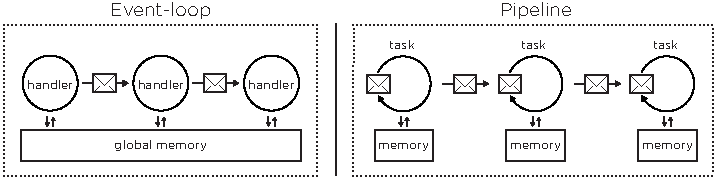
\includegraphics[page=1]{../resources/models-difference.pdf}}{
    \includegraphics[page=2]{../resources/models-difference.pdf}}{
  }
\end{figure}

% \begin{figure}
%   \centering
%   \textfig{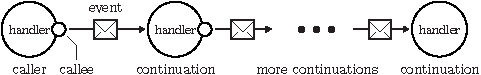
\includegraphics[width=0.8\linewidth]{../resources/cont-chain.pdf}}
% \end{figure}

\paragraph{Fluxional execution model}

The fluxional execution model is targeted by a more efficient programming language.
It executes an application expressed as a network of independent application parts called fluxions.
The fluxions communicate by messages, and form a pipeline similarly to the handlers of the event-driven execution model.
They are executed in parallel to distribute the computation across several cores and increase the performance efficiency.
They rely on isolated memory store, called context to allow this parallel execution.
When several fluxions need to rely on the same memory store, they are grouped, and executed sequentially.
When they are independent, they are isolated to increase performance efficiency.

The similarity between the event-driven execution model and the fluxional execution model leads to the equivalence presented in the next paragraph.
With this equivalence, the versatility of fluxions allows to progressively adapt the implementation from a productive, single event-loop, toward an efficient pipeline.

\subsection{Equivalence}

The equivalence describes the transformation from an application targeting the event-driven execution model to execute them in parallel in the fluxional execution model.
This transformation involves two steps: the extraction and isolation of the stages to form the pipeline.

\paragraph{Stage Extraction} \label{chapter7:summary:extraction}

The first step is the identification and extraction of the stages.
The equivalence identifies rupture points between stages.
A rupture point is an asynchronous call without subsequent synchronization with the caller.
It indicates a rupture in the synchronous control-flow, and the boundaries between two handlers.
The upstream handler is the one calling the asynchronous call, the downstream handler is the callback provided to the asynchronous call.

There are two kinds of rupture points: \textit{start} and \textit{post}.
\textit{Start} rupture points directly receives the input stream, and start the execution of the chain of stages for each new datum in the stream.
\textit{Post} rupture points indicates a continuity in the chain of stages.

The difficulty in this compilation step is to identify the asynchronous functions indicating the stages.
Because of the dynamic behaviors of Javascript, it is impossible to statically detect these functions.
The compiler implemented from the equivalence is currently unable to reliably detect them.
Instead the compiler rely on the developer to provide a list of asynchronous function names to extract.

\paragraph{Stage Isolation} \label{chapter7:summary:isolation}

% After the extraction of this pipeline,
The second step is the identification of the memory interdependencies between stages.
It intends to isolate the stages so they can be executed in parallel.
The common memory is replaced by message-passing, following some rules to preserve consistency.
\begin{itemize}
\item If a stage needs to hold a variable from one request to the other, this variable is stored in its context.
\item If a downstream stage needs to read a variable from an upstream stage, the variable is sent as part of the message communication.
\item If two stages needs to share a variable, they are grouped on the same execution node to safely share parts of their context.
Their executions are not parallelized to avoid conflicting accesses.
\end{itemize}

The difficulty in this step is to identify the memory dependencies between stages.
The dynamic behaviors of Javascript makes it impossible to statically identify aliasing in the memory.
The compiler implemented from the equivalence is currently unable identify these interdependencies.
It relies on manual manipulations to complete the transformation.

\separator

These difficulties are details in further details in the next section.
It then presents some perspectives to overcome these limitations.
\subsection{Real test case} \label{chapter5:flx:evaluation}

The compiler is tested on a real application, gifsockets-server\ftnt{https://github.com/twolfson/gifsockets-server}.
This test proves the possibility for an application to be compiled into a network of independent parts.
It shows the current limitations of this isolation and the modifications needed on the application to circumvent them.

\begin{code}[js, caption={Simplified version of gifsockets-server},label={lst:gifsocket}]
var express = require('express'),
    app = express(),
    routes = require('gifsockets-middleware'), //@\label{lst:gifsocket:gif-mw}@
    getRawBody = require('raw-body');

function bodyParser(limit) { //@\label{lst:gifsocket:bodyParser}@
  return function saveBody(req, res, next) { //@\label{lst:gifsocket:saveBody}@
    getRawBody(req, { //@\label{lst:gifsocket:getRawBody}@
      expected: req.headers['content-length'],
      limit: limit
    }, function (err, buffer) { //@\label{lst:gifsocket:callback}@
      req.body = buffer;
      next(); //@\label{lst:gifsocket:next}@
    });
  };
}

app.post('/image/text', bodyParser(1 * 1024 * 1024), routes.writeTextToImages); //@\label{lst:gifsocket:app.post}@
app.listen(8000);
\end{code}

This application, simplified in listing \ref{lst:gifsocket}, is a real-time chat using gif-based communication channels.
It was selected from the evaluation set of the Due compiler because it is simple enough to illustrate this evaluation.
% \cite{Brodu2015}
%  from the \texttt{npm} registry because it depends on \texttt{express}, it is tested, working, and simple enough to illustrate this evaluation.
The server transforms the received text into a gif frame, and pushes it back to a never-ending gif to be displayed on the client.

On line \ref{lst:gifsocket:app.post}, the application registers two functions to process the requests received on the url \texttt{/image/text}.
The closure \texttt{saveBody}, line \ref{lst:gifsocket:saveBody}, returned by \texttt{bodyParser}, line \ref{lst:gifsocket:bodyParser}, and the method \texttt{routes.write\-Text\-To\-Images} from the external module \texttt{gifsockets-\-middleware}, line \ref{lst:gifsocket:gif-mw}.
The closure \texttt{saveBody} calls the asynchronous function \texttt{getRawBody} to get the request body.
Its callback handles the errors, and calls \texttt{next} to continue processing the request with the next function, \texttt{routes.write\-Text\-To\-Images}.

\subsubsection{Compilation} \label{chapter5:flx:evaluation:compilation}

% We compile this application with the compiler
The compilation result is in listing \ref{lst:flx-gifsocket}.
The function call \texttt{app.post}, line \ref{lst:gifsocket:app.post}, is a rupture point.
However, its callbacks, \texttt{bodyParser} and \texttt{routes.write\-Text\-To\-Images} are not declared \textit{in situ}.
They are evaluated as functions only at runtime.
As precised previously, the compiler discards these callbacks to avoid altering the semantic. % by moving or modifying their definition.
% For this reason, the compiler ignores this rupture point, to avoid interfering with the evaluation.

\begin{code}[flx, caption={Compilation result of gifsockets-server},label={lst:flx-gifsocket}]
flx main & express {req}
>> anonymous_1000 [req, next]
  var express = require('express'),
      app = express(),
      routes = require('gifsockets-middleware'), //@\label{lst:flx-gifsocket:gif-mw}@
      getRawBody = require('raw-body');

  function bodyParser(limit) { //@\label{lst:flx-gifsocket:bodyParser}@
    return function saveBody(req, res, next) { //@\label{lst:flx-gifsocket:saveBody}@
      getRawBody(req, { //@\label{lst:flx-gifsocket:getRawBody}@
        expected: req.headers['content-length'], //@\label{lst:flx-gifsocket:req.headers}@
        limit: limit
      }, >> anonymous_1000 [req, next]);
    };
  }

  app.post('/image/text', bodyParser(1 * 1024 * 1024), routes.writeTextToImages); //@\label{lst:flx-gifsocket:app.post}@
  app.listen(8000);

flx anonymous_1000
-> null
  function (err, buffer) { //@\label{lst:flx-gifsocket:callback}@
    req.body = buffer; //@\label{lst:flx-gifsocket:buffer}@
    next(); //@\label{lst:flx-gifsocket:next}@
  }
\end{code}

The compiler detects a rupture point : the function \texttt{get\-Raw\-Body} and its anonymous callback, line \ref{lst:gifsocket:callback}.
It encapsulates this callback in a fluxion named \texttt{anony\-mous\_\-1000}.
The callback is replaced with a stream placeholder to send the message stream to this downstream fluxion.
The variables \texttt{req} and \texttt{next} are appended to this message stream, to propagate their value from the \texttt{main} fluxion to the \texttt{anony\-mous\_\-1000} fluxion.

When \texttt{anony\-mous\_\-1000} is not isolated from the \texttt{main} fluxion, as if they belong to the same group, the compilation result works as expected.
The variables used in the fluxion, \texttt{req} and \texttt{next}, are still shared between the two fluxions.
In this situation fluxions are quite similar to Dues regarding memory shareing.
Our goal is to isolate the two fluxions, to be able to safely parallelize their executions.

\subsubsection{Isolation} \label{chapter5:flx:evaluation:isolation}

In listing \ref{lst:flx-gifsocket}, the fluxion \texttt{anony\-mous\_\-1000} modifies the object \texttt{req}, line \ref{lst:flx-gifsocket:buffer}, to store the text of the received request, and it calls \texttt{next} to continue the execution, line \ref{lst:flx-gifsocket:next}.
\texttt{req} is an alias to a memory location used in multiple palces in code.
Therefore, these operations produce side-effects that should propagate in the whole application, but the isolation prevents this propagation.
Isolating the fluxion \texttt{anony\-mous\_\-1000} produces runtime exceptions.
The next paragraph details how this situation is handled to allow the application to be parallelized.

\paragraph{Variable \texttt{req}}

The variable \texttt{req} is read in fluxion \texttt{main}, lines \ref{lst:flx-gifsocket:getRawBody} and \ref{lst:flx-gifsocket:req.headers}.
Then its property \texttt{body} is associated to \texttt{buffer} in fluxion \texttt{anony\-mous\_\-1000}, line \ref{lst:flx-gifsocket:buffer}.
The compiler is unable to identify the aliases of this variable. % further usages.
However, the side effect resulting from this association impacts a variable in the scope of the next callback, \texttt{routes.write\-Text\-To\-Images}.
In this test case, the application is modified manually to explicitly propagate this side-effect to the next callback through the function \texttt{next}.
The modifications of this function are explained further in the next paragraph.

\paragraph{Closure \texttt{next}}

The function \texttt{next} is a closure provided by the \texttt{express} \texttt{Router} to continue the execution with the next function to handle the client request.
Because it indirectly relies on the variable \texttt{req}, it is impossible to isolate its execution with the \texttt{anony\-mous\_\-1000} fluxion.
Instead, we modify \texttt{express}, so as to be compatible with the fluxional execution model.
We explain the modifications below.

\begin{code}[flx, caption={Simplified modification on the compiled result},label={lst:mflx-gifsocket}]
flx anonymous_1000
-> express_dispatcher
  function (err, buffer) { //@\label{lst:mflx-gifsocket:callback}@
    req.body = buffer; //@\label{lst:mflx-gifsocket:buffer}@
    next_placeholder(req, -> express_dispatcher); //@\label{lst:mflx-gifsocket:next-placeholder}@
  }

flx express_dispatcher & express {req} //@\label{lst:mflx-gifsocket:express-dispatcher}@
-> null
  function (modified_req) {
    merge(req, modified_req);
    next(); //@\label{lst:mflx-gifsocket:next}@
  }
\end{code}

In listing \ref{lst:gifsocket}, the function \texttt{next} is a continuation allowing the anonymous callback, line \ref{lst:gifsocket:callback}, to call the next function to handle the request.
To isolate the anonymous callback into \texttt{anonymous\_\-1000}, \texttt{next} is replaced by a rupture point.
This replacement is illustrated in listing \ref{lst:mflx-gifsocket}.
The \texttt{express} \texttt{Router} registers a fluxion named \texttt{express\_\-dispatcher}, line \ref{lst:mflx-gifsocket:express-dispatcher}, to continue the execution after the fluxion \texttt{anony\-mous\_\-1000}.
This fluxion is in the same group \texttt{express} as the \texttt{main} fluxion, hence it has access to the original variable \texttt{req}, and to the original function \texttt{next}.
The call to the original \texttt{next} function is replaced by a placeholder to push the stream to the fluxion \texttt{express\_\-dispatcher}, line \ref{lst:mflx-gifsocket:next-placeholder}.
The fluxion \texttt{express\_\-dispatcher} receives the stream from the upstream fluxion \texttt{anony\-mous\_\-1000}, merges back the modification in the variable \texttt{req} to propagate the side effects, and finally calls the original function \texttt{next} to continue the execution, line \ref{lst:mflx-gifsocket:next}.

After the modifications detailed above, the server works as expected.
The isolated fluxion correctly receives, and returns its serialized messages.
The client successfully receives a gif frame containing the text.



\subsection{Limitations}

The static analysis used for this compiler presents some limitations.
It is unable to analyze code with dynamic behaviors.
Higher-order programming leads to more productivity partly beacuse it rely on such dynamic behavior to extend expressivity.
Precisely, it allows more levels of indirections.

\subsubsection{Levels of Indirections}

The indirection is an abstraction between the value, and its manipulation.
In listing \ref{lst:indirection}, the variables \texttt{a} and \texttt{b} point both to the same memory object.
The function \texttt{fn} introduces a level of indirection between the real object \texttt{a} and its manipulation handle, \texttt{b};
% Actually, the variable \texttt{a} already introduces a level of indirection between the real object and the handle \texttt{a}.

\begin{code}[js,
  caption={One level of Indirection},
  label={lst:indirection}]
var a = {
      // an object;
    };

fn(b) {
  // modify b;
}

fn(a);
\end{code}

\subsubsection{Uncertainties}

The indirection is trivial to resolve in listing \ref{lst:indirection}.
It only needs to have access to the definition of \texttt{a} and of \texttt{fn}.
%A very simple static analysis could resolve it.
However, in listing \ref{lst:indirections}, the array \texttt{handlers} introduces a new level of indirection.
The static analysis now needs to have access to the definition of \texttt{i} and of the \texttt{handlers}.
If this definition is provided by an external input, it is not available statically, hence, it adds an uncertainty during the analysis. 

\begin{code}[js,
  caption={Two levels of indirection},
  label={lst:indirections}]
var a = {
      // an object;
    },
    handlers = [
      // definition of fn handlers;
    ],
    i = ?;

handlers[i](a);
handlers[i+1](a);
\end{code}

These examples are extremely simplified.
A real application contains enough indirections for the static analysis to be overwhelmed by uncertainties, and to be unable to resolve the variables.
If a variable is left unresolved, it is impossible to assure its scope and its aliases.
Therefore, the compiler is unable to isolate it into a fluxion, or to distribute its modification by messages.

Moreover, it leads the compiler to ignore the rupture points not defined \textit{in situ}, because their modifications could impact the semantic.
The reason for this precaution, is that the compiler is unable to assure where the function is used, and the scope of its variables.
Therefore, it is unable to assure that the modification will conserve the semantic.

\subsubsection{Dynamic Resolution}

In a web application, this variable \texttt{i} might be part of the user request, which is available only at runtime.
It eventually introduces an uncertainty.

This dynamic resolution of variables is precisely what increase expressiveness.
Trying to resolve them statically is equivalent to restrict expressiveness.
No static analysis can overstep these limitations.
Only a dynamic analysis could analysis the resolved indirections during run time to overstep these limitations correctly.



\section{Perspectives} \label{chapter6:perspective}

As stated previously, static analysis impacts productivity to favor efficiency.
% For example, to isolate fluxions, the current implementation of the compiler restrains the developer to use only \textit{in situ} callbacks, and avoids aliasing.
Though, an interesting perspective to continue this work is to implement as a just-in-time compiler.
Indeed, the dynamic analysis allowed at run time is more prone to overcome the limitation identified with static analysis.

\subsection{Just-in-time Compilation}

Most Javascript interpreters compile some parts of the code at run time to improve performances.
During this compilation, the levels of indirections are mostly resolved.
The code is translated directly into lower-level instructions.

Implementing the equivalence in a just-in-time (JIT) compiler could leverage this dynamic resolution.
It could analyze the scope of variables resolved dynamically, and isolate the stages accordingly.

\paragraph{Rupture point detection}

The asynchronous functions identifying rupture points are not part of Javascript.
They are special functions provided by the interpreter.
With the compiler communicating with the interpreter at run time, detecting rupture points become trivial.
The interpreter notifies the compiler when an asynchronous function is called.
The compiler then identifies the rupture point and isolates it to possibly execute it remotely.

\paragraph{Dominator Tree}

To debug the memory in dynamic languages like Javascript, one can use a dominator tree.
It is a tree generated at run time indicating the parenting relations between memory objects.
With such a tree, the analysis of interdependencies between stages becomes trivial.
Each stage can be isolated in a fluxion, and deployed accordingly to its dependencies.

% With the dynamic registering of Fluxions to the messaging system, and into tag groups, it is possible to transform a Javascript application continuously during its execution.
% Analysis of the interdependencies become as trivial as for static languages, with the resolution of the indirections by the just-in-time compiler.
% The fluxional compiler waits for these resolutions, and then analyzes the compiled code for rupture points.
% As the asynchronism of a function call is handled by the execution engine, the just-in-time compilation can pin point precisely the asynchronous calls from the synchronous ones. 
% And the continuations for these asynchronous calls are resolved, which makes them similar to inline continuations.

\paragraph{Closure Serialization}

Closures are required to allow higher-order programming.
But the static compiler is unable to manipulate closures, as illustrated in section \ref{chapter5:flx:evaluation:isolation}.
Closures are generated dynamically by the interpreter.
With the compiler communicating with the interpreter, the former can manipulates and serialize them at run time.
It can then send closures between fluxions, like any other objects.
It enables the use of higher-order programming within the fluxional execution model.
Hence, it would allow, to some extent, to improve the compromise between productivity and efficiency.
Indeed, the developer is free to use the higher-order programming to compose modules, with a global memory abstraction.
Yet, the execution could distribute this global memory abstraction according to the detected interdependencies.

\paragraph{Dynamic Grouping}

With the dynamic detection of stages and their dependencies, and the manipulation of closures, fluxions can be registered during the execution of the application.
To assure they meet their dependencies, the fluxions are deployed according to their groups.
Two fluxions belong to the same group if they need to share access to some variables.
Therefore, they need to be deployed on the same event-loop to share their memory.

\paragraph{Safe-Checking}

It is required to safe-check that the compiled code is consistent with the remaining execution.
As an example, just-in-time compilers check the type to assure that a compiled function remains conform to the input and output types of its call site.
Similarly, it is required to check that the deployment of fluxions doesn't cause inconsistencies.

If a fluxion ready to be deployed belongs to two different groups, these two groups needs to be gathered on the same event-loop.
If they were previously deployed on two different event-loops, they need to be moved with their context to be on the same event-loop.
Moreover, to assure consistency, they need to be moved when receiving the request that triggered the fluxion ready to be deployed.
So that when this new fluxion is executed at this message reception it has access to the contexts of the two groups.
For this purpose, the compiler put the execution on hold, and sends a control message downstream to order the move of the fluxions.
% It interleaves control messages in the stream to communicate with the distributed interpreters.
In this example, the message inquired the distributed interpreters to stop execution, pack the fluxions and their contexts, and send them back to another remote interpreter.
To assure consistency, the execution resumes only when all the fluxions are gathered in the same event-loop, with access to the whole shared memory.

% If the new fluxion depends an a local variable, as well as a variable from a group on another node than the local node, the group needs to be deployed back locally.
% The fluxion as well as all the fluxions of the group are deployed locally, but the execution needs to wait for the contexts of the group to be available locally.
% To gather the contexts, the node responsible for this group send a message to the messaging system managing this group.
% The messaging system gather all the contexts of the fluxions, and send them back.
% When the contexts are deployed locally to the new node responsible for the this group, the execution of this branch can resume.

% A new compromise have to be done between the cost of sending a fluxion and the cost to get it back, and the risk that it requires to be sent back.
% It might be possible to reduce this risk by saving the compilation information from one execution to the other.

\separator

The perspectives described in the previous paragraphs overcome the limitations of the current implementation of the compiler.
They describe the further implementation of the equivalence, as if I were to continue this work.

\subsection{Evaluation of the perspective}

This second evaluation admits that the JIT compilation resolves all the indirections in the memory.
% Which is left unknown after this thesis.
Then, the fluxional JIT compiler doesn't need to rely on human interaction.
Therefore, the expected productivity is the same as the productivity language used as source. %, as illustrated in table \ref{tab:perspective-productivity}.

% \TablePerspectiveProductivity{tab:perspective-productivity}

Naturally, the performance efficiency of the implementation is, at first, the same of this productivity language, as the development is focused on productivity.
Some development efforts are required to improve the efficiency.
% But the result of the compilation helps in this shift.
The result from the compiler helps the developer find the bottle necks, and reduce the effort for this shift.
With the help from the compiler, the effort for this shift is expected to be less than the current required effort.
% The effort for this shift are expected to be less than the current required effort. %, as illustrated in table \ref{tab:perspective-efficiency}.
Instead of redesigning the architecture of the application to immediately isolate components, it is possible to modify them to progressively loosen their dependencies.
As illustrated in table \ref{tab:perspective-summary}, this envisioned platform is expected to yield both productivity and efficiency, not at the same time, but when they are required the most.

% \TablePerspectiveEfficiency{tab:perspective-efficiency}

Moreover, during this decomposition and after, developers can still rely on higher-order programming, even between isolated application parts.
In the current state of the art, there is no known platform to offer higher-order programming between distributed parts.
This possibility is therefore unknown, and could actually yield to an unrivaled compromise between productivity and efficiency.

Following the insight along this thesis, a platform bringing both productivity and efficiency simultaneously would be greatly adopted.
But it requires to be observed in real conditions before drawing this conclusion.
% , as illustrated in table \ref{tab:perspective-adoption}.

% \TablePerspectiveAdoption{tab:perspective-adoption}
% \separator

\TablePerspectiveSummary{tab:perspective-summary}

\subsection{Final Thoughts}

As I studied for this thesis, I progressively saw the world differently.
And as a final note in this thesis, I want to share this view.

\paragraph{Economic Considerations}

The IT industry understood that trading efficiency for productivity could reduce development time and cost, and hardware performance could compensate.
This thesis intends to bring a reconciliation between two economical concerns in the development of a web application, the efficiency of execution and the productivity of development.
I believe that it is time to take into account both productivity and efficiency.

The IT industry has an important impact on the environment with its increasing carbon footprint.
As the digitalization permeates into every aspects of our lives, it is of crucial importance to consider this impact.
Therefore, it is time to reduce the efficiency to the minimum required.
Yet, with the increasing importance of the IT, development cannot be reserved to experts anymore.
Productivity cannot be traded back for efficiency.

% I leave for future works the reconciliation of the efficiency of energy consumption with the two concerns addresses in this thesis.
% Like with ThinkAir and Maui, whete the code offloading can helps to save energy on the mobile \cite{Kosta2012,Cuervo2010a}.

\paragraph{Accessible And Omnipresent Development}

This epoch feels like developers are the scribes and the monks after the invention of writing.
I believe that in the time to come, development will be made available for everybody.
And additionally as reading and writing, developing will be a prerequisite to communicate with peers.
It will allow to express dynamic behaviors, and not only static ones, as Bret Viktor already envisioned\ftnt{https://vimeo.com/115154289}.

This shift might come with the increasing importance of machine learning.
Indeed, it allows to define complex dynamic behaviors without specifically describing every corner cases.
It feels like the composition of general case behavior that can seamlessly meld at corner cases.
If machine learning can become parts of our daily means of communication, it will radically change our interactions with peers, and with the world.

Moreover, with the advent of the smart contracts based on block chain technology, and the Internet of things, it is not far-fetched to imagine our everyday world infused with behaviors defined by others.
I believe the difference between a person and its environment will start to dissolve.
A limited preview can be drawn in our dependence to Internet, smart-phones and other connected objects.
But the possibilities are beyond our current imagination.

\paragraph{Scalability}

At the light of this thesis, I understand that scalability boils down to the choice of an organization.
The chosen organization determines what should be kept local, versus, what should be spread globally.
I believe the same problematic applies to many different everyday organizations, such as economical and social organizations.

For example, in economy, it is important for certain markets to spread globally.
The different international markets, such as stocks and foreign currency exchange market, are crucial to spread economical informations worldwide.
The variations of prices on these markets yields the informations to direct the consumption and production of every product and raw materials for the entire population.
It avoids spoiling resources.
On the contrary, the uncontrolled variations of this global economy can be destructive at a wide scale, and must somehow be contained.
Local citizen currency is an example of such containment.
It contains the scope of these variations within a local region.

To concludes this thesis, I yield the following problematic.
How to layout the organizations composing our everyday world for it to be efficient.
Economically, socially, and in many other aspect of our everyday lives, I believe designing an efficient organization boils down to choosing which piece of information shall be kept locally, or spread globally.